% Paper 2015
\documentclass[peerreviewca,11pt,a4paper]{IEEEtran}

\usepackage{ifpdf}
\usepackage{cite}

\ifCLASSINFOpdf
    \usepackage[pdftex]{graphicx}
    \graphicspath{{../pdf/}{../jpeg/}}
    \DeclareGraphicsExtensions{.pdf,.jpeg,.png}
\else
    \usepackage[dvips]{graphicx}
    \graphicspath{{../eps/}}
    \DeclareGraphicsExtensions{.eps}
\fi

\usepackage[cmex10]{amsmath}

\usepackage{array}
\usepackage{fixltx2e}

\ifCLASSOPTIONcaptionsoff
  \usepackage[nomarkers]{endfloat}
 \let\MYoriglatexcaption\caption
\renewcommand{\caption}[2][\relax]{\MYoriglatexcaption[#2]{#2}}
\fi

\usepackage{url}

\usepackage{siunitx}
\DeclareSIUnit\photon{\ensuremath{\gamma}}
\DeclareSIUnit\proton{p}
\DeclareSIUnit\neutron{n}

\usepackage{booktabs}

\usepackage{graphicx}
\usepackage{epstopdf}

\usepackage{caption}
\usepackage{subcaption}

\usepackage{todo}
%\renewcommand\todo[1]{\relax}
%\renewcommand\todos{\relax}

\usepackage{bpchem}
\def\U238{\BPChem{\^{238}U}}

% correct bad hyphenation here
\hyphenation{op-tical net-works semi-conduc-tor}

\begin{document}

\title{
    Detailed Geant4 simulations of the ANITA and ANITA-CUP neutron facilities
}

\author{
    \IEEEauthorblockN{
        Q. Hong\IEEEauthorrefmark{1},
        S. P. Platt\IEEEauthorrefmark{1},
        A. V. Prokofiev\IEEEauthorrefmark{2} and
        E. Passoth\IEEEauthorrefmark{2}
    }
    \IEEEauthorblockA{
        \IEEEauthorrefmark{1}
        University of Central Lancashire
    }
    \IEEEauthorblockA{
        \IEEEauthorrefmark{2}
        The Svedberg Laboratory, University of Uppsala
    }
}

\maketitle

\begin{abstract}
    Monte Carlo simulation of spallation neutron source of ANITA at TSL was used to analyze radiation fields at the Close User Position (CUP) and Standard User Position(SUP) for single-event effect testing. ...
    \todo{Revise abstract}
\end{abstract}

\IEEEpeerreviewmaketitle

\section{Introduction}

The ANITA facility at The Svedberg Laboratory has been widely used for accelerated testing for neutron single-event effects (SEE)~\cite{Prokofiev2009}.
A high-flux facility, ANITA-CUP, has recently been introduced and reported by Prokofiev et al.~\cite{Prokofiev2014}.

Platt et al. have reported preliminary Monte Carlo models of neutron and gamma production at ANITA~\cite{Platt2013}.
That work was motivated by a desire to understand the possibility of gamma sensitivity in detectors used for beam monitoring during SEE tests.
Simulations of a bare spallation target showed qualitative agreement with independent calculations and measurements of the fast neutron field at the standard ANITA facility.
The present work was motivated partly by a desire to investigate whether improvements in the fidelity of the geometry used in the simulations would lead to closer quantitative agreement with independent data, and partly to extend the work to encompass the new facility at ANITA-CUP.

Accordingly, in this paper we will present a comprehensive set of analyses of neutron and gamma fields at ANITA and ANITA-CUP, with comparison against independent models and validation against measurements.
We present a subset of those results in this extended abstract.

\section{Modelling}
Simulations were conducted using Geant4 version 10.0~\cite{Agostinelli2003,Allison2006} with the binary intranuclear cascade model~\cite{Platt2013}.
A detailed model of the ANITA geometry~\cite{Prokofiev2009,Prokofiev2014} was implemented in Geant4, as illustrated in Fig.~\ref{fig:ANITAoverview}.
%; a summary only is given here.
%The spallation target is a tungsten cylinder of diameter \SI{5}{\cm} and length \SI{2.4}{\cm}~\cite{ANITAdrawing}.
%The target is cooled by water and surrounded by a stainless-steel cooling jacket.
%The target assembly with its cooling jacket appears as a small blue rectangle in Fig.~\ref{fig:ANITAoverview}.
%Lead shielding blocks in the target region are also modelled, and shown in red Fig.~\ref{fig:ANITAoverview}.
%A large electromagnet surrounding the target is modelled and shown in Fig.~\ref{fig:ANITAoverview} in grey (iron) and yellow (copper).
%An iron collimator with variable apertures is modelled  and shown downstream of the target (grey).
Simulated protons were incident axially at an energy of \SI{180}{\MeV}.
Resulting neutron and gamma fields were evaluated at several detector locations.
In this paper results are presented for three of these: the Standard User Position (SUP), \SI{2.5}{\m} downstream of the target, the Close User Position (CUP), \SI{0.75}{\m} downstream of the target, and the CUP-TOF, \SI{0.84}{m} downstream of the target.
%N.B. This is downstream of the downstream edge of the target in Qian's model.
The SUP position is downstream of a collimator with variable aperture; the CUP and CUP-TOF positions are upstream of the same collimator.
The SUP and CUP positions are of interest as they are positions used for SEE tests; the CUP-TOF position is the location of thin-film breakdown counter (TFBC) detectors used for beam monitoring and characterisation.
TFBC data are used to validate simulation results.

\begin{figure}[t]
	\centering
	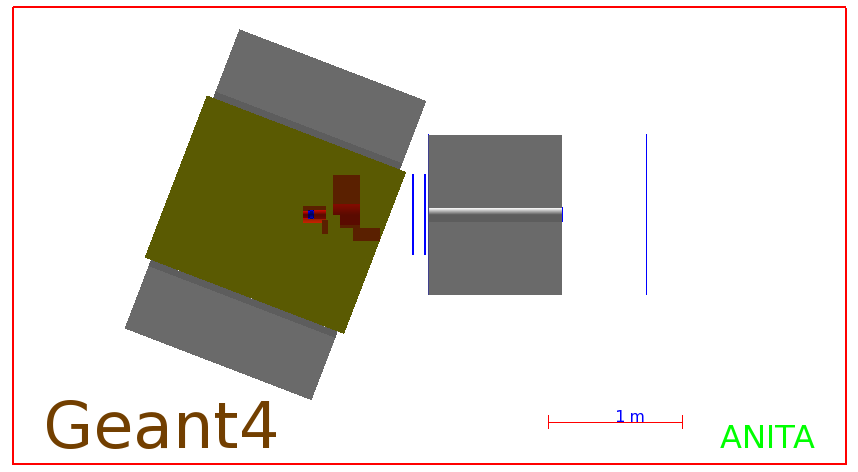
\includegraphics[width=\columnwidth]{overview.png}
	\caption{
        Simulated ANITA facility overview seen from above (yellow: bending magnet; red: shielding components; blue: target assembly; grey: collimator; blue: detector system)
    }
	\label{fig:ANITAoverview}
\end{figure}

\section{Results}

\subsection{Neutrons}
Fig.~\ref{fig:SUPDensity} shows neutron spatial distribution at the SUP, for neutrons above \SI{10}{\MeV}.
Collimation is clearly visible.
Within the beam umbra the calculated neutron fluence rate above \SI{10}{\MeV} at a proton current of \SI{200}{\nA} is \SI{7.1e5}{\neutron\per\cm\squared\per\second}, compared to \SI{5.7e5}{\neutron\per\cm\squared\per\second} from earlier calculations~\cite{Platt2013} and \SI{9.3e5}{\neutron\per\cm\squared\per\second} from an established analytical model~\cite{Prokofiev2009}.
The analytical model therefore exceeds the present calculations by about 30\%.

\begin{figure}[t]
    \begin{minipage}{\columnwidth}
        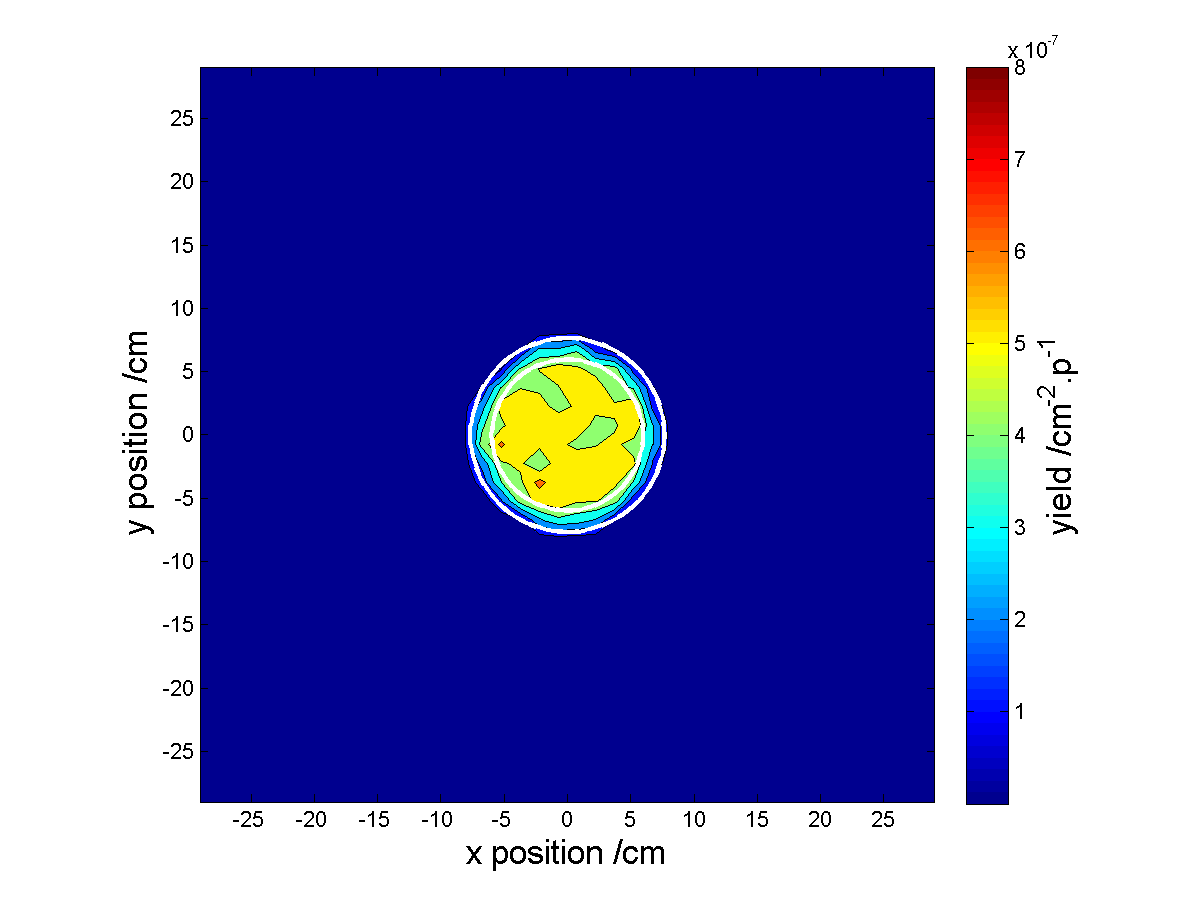
\includegraphics[width=\columnwidth]{SUP10ColSpatialDistribution10MeVRADECS.png}
        \subcaption{
            Standard User Position.
            Concentric white circles indicate nominal umbra and penumbra limits
        }
        \label{fig:SUPDensity}
    \end{minipage}
    \begin{minipage}{\columnwidth}
        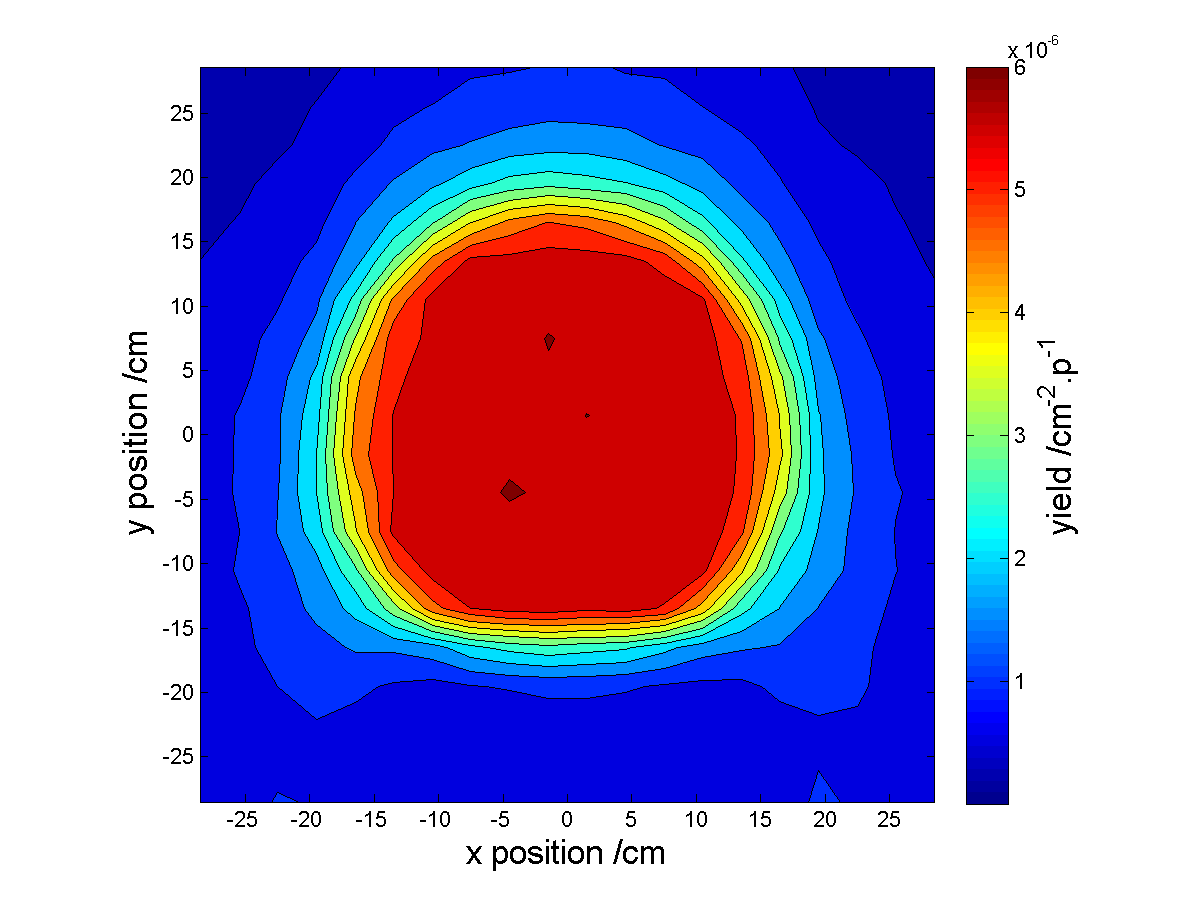
\includegraphics[width=\columnwidth]{CUP10ColSpatialDistribution10MeV.png}
        \subcaption{Close User Position}
        \label{fig:CUPDensity}
    \end{minipage}
    \caption{
        Spatial distribution of neutrons above \SI{10}{\MeV} at SUP and CUP, with \SI{10.2}{\cm} diameter collimator
    }
\end{figure}

Fig.~\ref{fig:CUPDensity} shows equivalent data for the CUP, which is upstream of the collimator.
In the central region the calculated neutron fluence rate above \SI{10}{\MeV} at a proton current of \SI{200}{\nA} is \SI{7.85e6}{\neutron\per\cm\squared\per\second}, compared to \SI{1.17e7}{\neutron\per\cm\squared\per\second} from an analytical model reported by Prokofiev et al.~\cite{Prokofiev2014}.
The analytical model therefore exceeds the present calculations about 50\%.
The results show\ldots
\todo{Describe the results: contours at CUP and SUP}

Fig.~\ref{fig:CUPProfile} shows neutron fluence profile at the CUP, compared with measurements made with \U238\ TFBCs.
Results of calculations were folded in energy with the neutron fission cross section for \U238~\cite{Carlson2009}.
The results show\ldots
\todo{Describe the results: profile at CUP}

\begin{figure}[t]
    \centering
    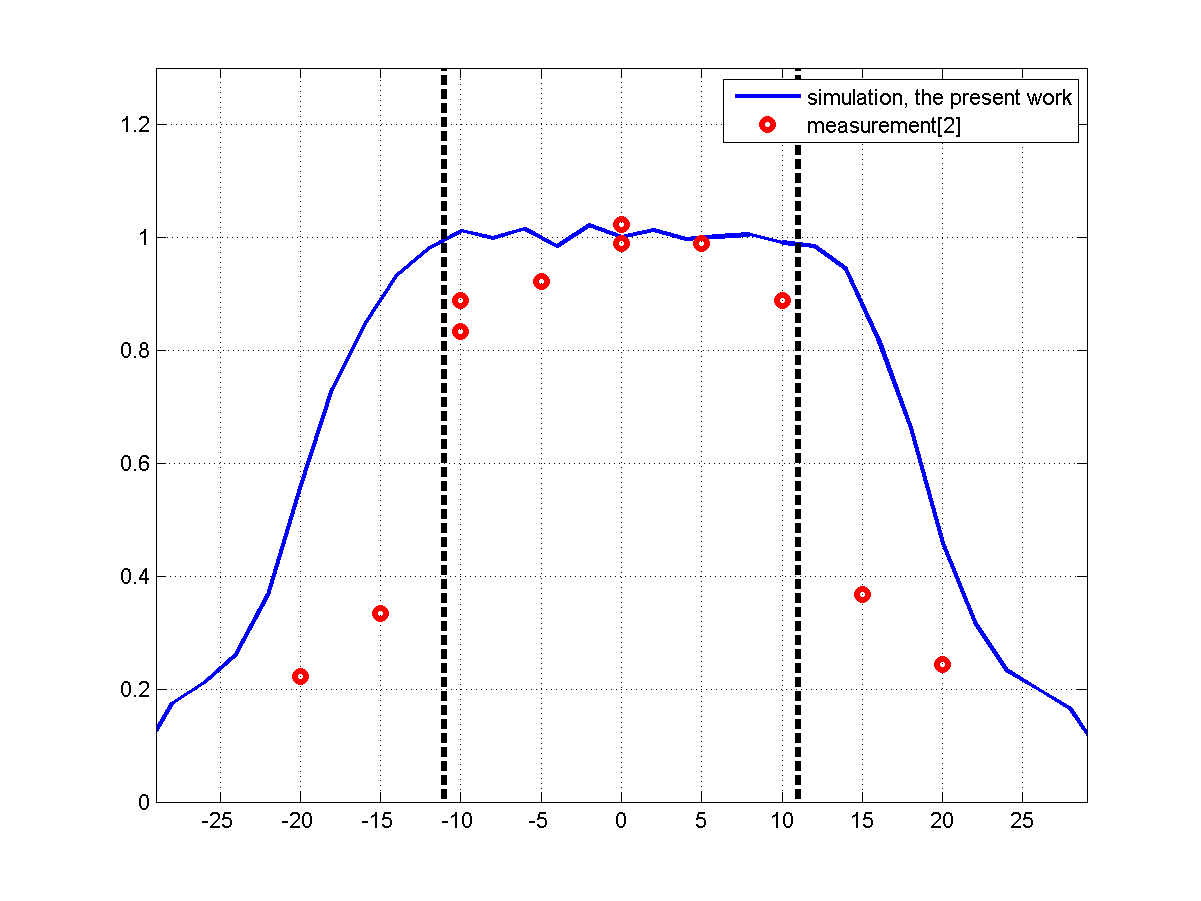
\includegraphics[width=\columnwidth]{CUPTOF10beamproRADECS.png}
    \caption{
        Neutron profile at the CUP, normalised to fluence rate on axis, with
        \SI{10.2}{\cm} diameter collimator}
    \label{fig:CUPProfile}
\end{figure}

Fig.~\ref{fig:TOFSpectra} compares simulated and measured TOF spectra at the CUP-TOF position.
Neutron time of flight data from the simulation were folded in energy with the \U238\ fission cross-section, convolved with a \SI{5}{\ns} rectangle function approximating the primary proton micropulse shape, and overlapped at \SI{45}{\ns}, representing the timing ambiguity due to the micropulse period.
The results show\ldots
\todo{Explain what the results show.}

\begin{figure}[t]
    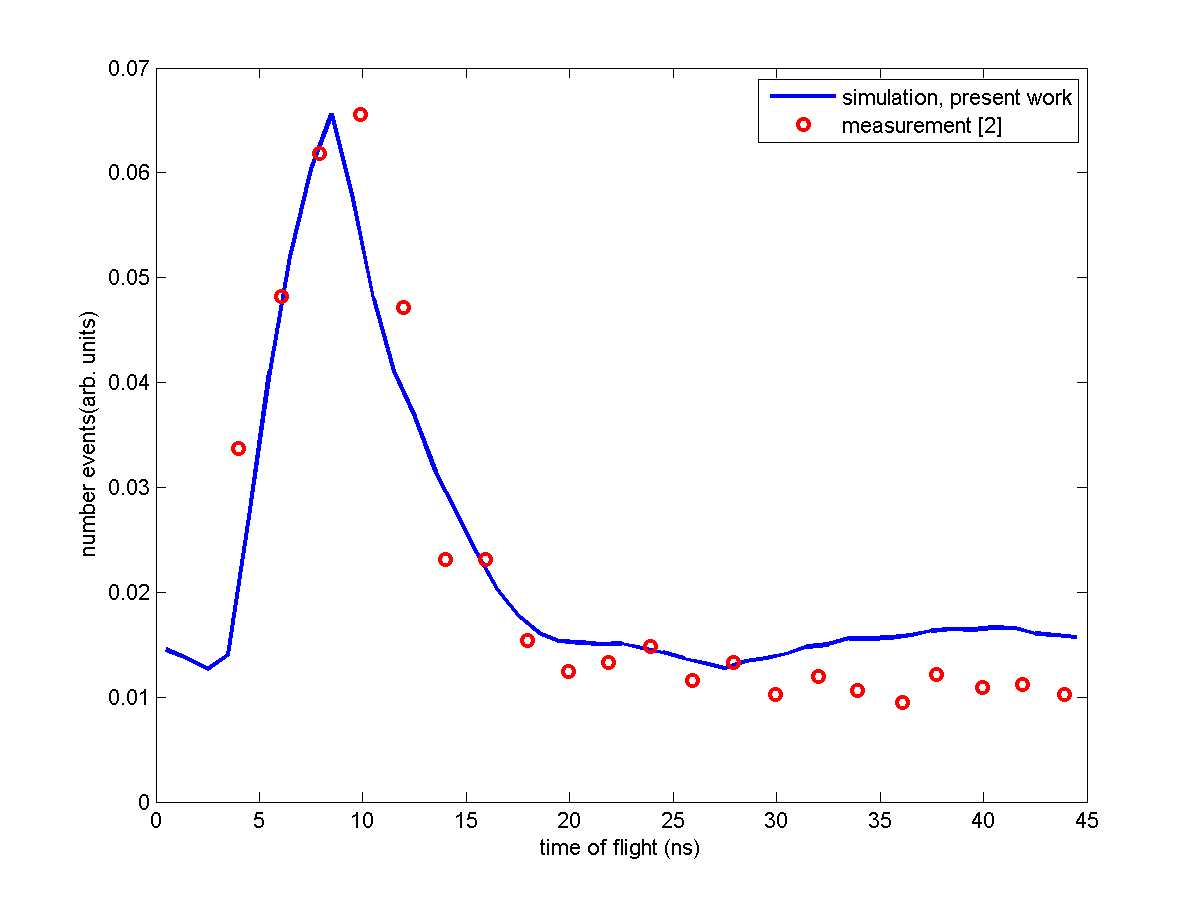
\includegraphics[width=\columnwidth]{CUPTOFtofspectraRADECS.png}
    \caption{
        Neutron time of flight spectra at the CUP-TOF position, with \SI{3}{\cm} diameter collimator
        }
    \label{fig:TOFSpectra}
\end{figure}

Fig.~\ref{fig:Lethargyplots} compares calculated spectra at SUP and CUP with their respective analytical models.
The SUP data are also compared with results from preliminary Geant4 simulations~\cite{Platt2013}.
The results show\ldots
\todo{Describe the neutron spectra.}

\begin{figure}[t]
    \begin{minipage}{\columnwidth}
        \centering
        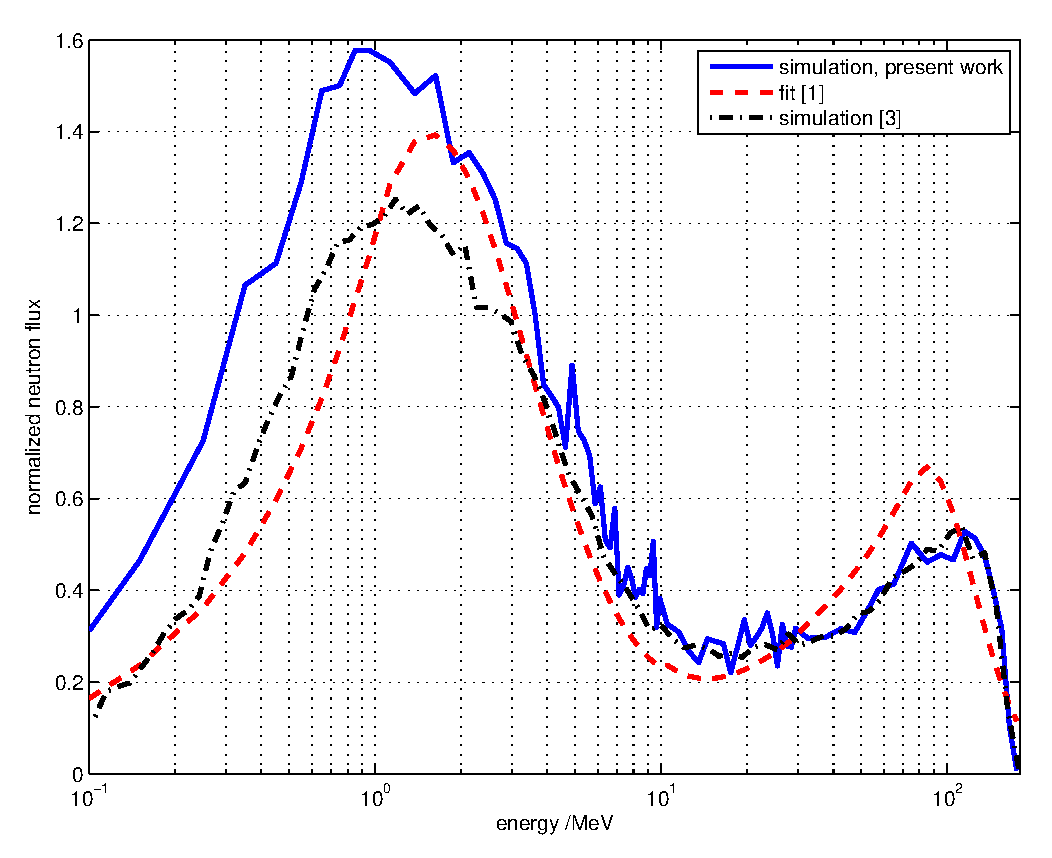
\includegraphics[width=0.9\columnwidth]{SUPNormalisedRADECS.eps}
        \subcaption{
            SUP.
            The comparison is against the fit of Prokofiev et al.~\cite{Prokofiev2009} and preliminary Geant4 modelling by Platt et al.~\cite{Platt2013} }
    \end{minipage}
    \begin{minipage}{\columnwidth}
        \centering
        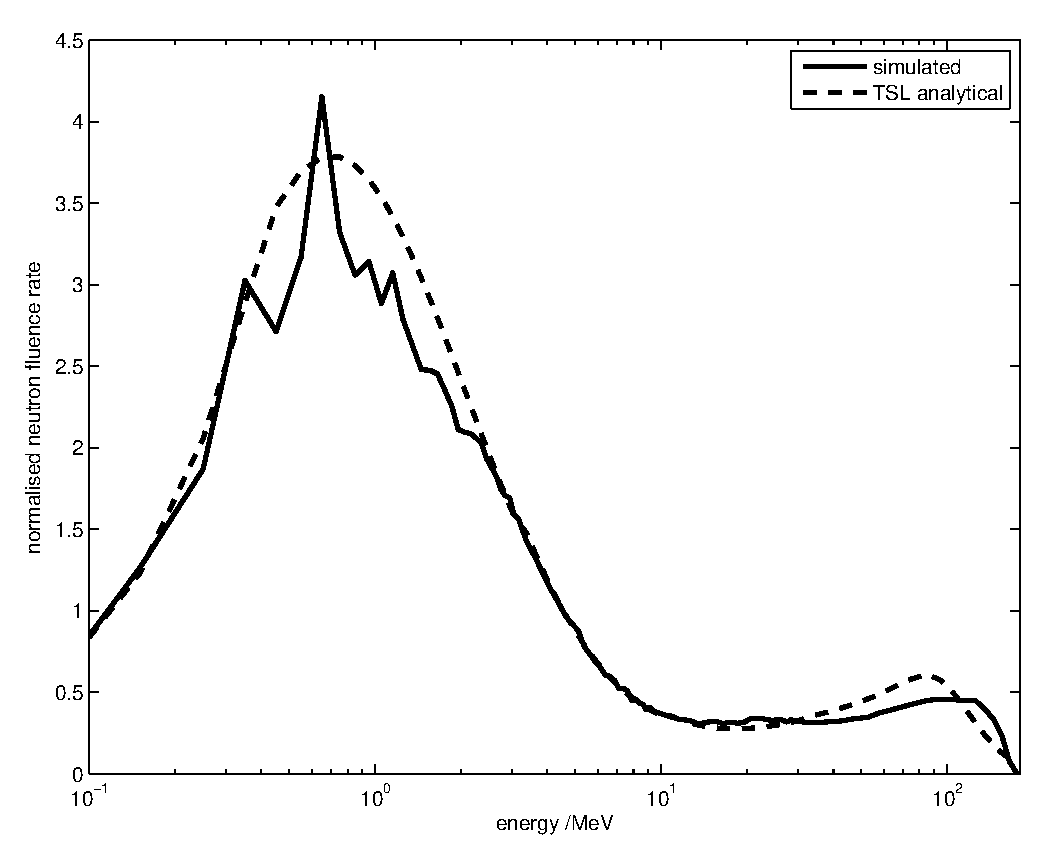
\includegraphics[width=0.9\columnwidth]{CUPcomparedProkofiev2014NormalisedRADECS.eps}
        \subcaption{
            CUP.
            The comparison is against the fit of Prokofiev et al.~\cite{Prokofiev2014}
        }
    \end{minipage}
	\caption{
        Calculated neutron spectra, normalised to fluence above \SI{10}{\MeV}, with
        \SI{10.2}{\cm} diameter collimator
    }
	\label{fig:Lethargyplots}
\end{figure}

Fig.~\ref{fig:DifferentialSpectra} summarises neutron spectra results by comparing differential flux as calculated in this work with the Prokofiev et al. models~\cite{Prokofiev2009,Prokofiev2014}.
The SUP calculations and analytical model agree very closely below \SI{20}{\MeV}; the analytical model exceeds the calculations somewhat above that energy.
At CUP the analytical model exceeds the Geant4 calculations by about 50\%, slightly more than that above \SI{20}{\MeV}.
\todo{Improve precision of the summary description of differential spectra.}

\begin{figure}[t]
    \centering
    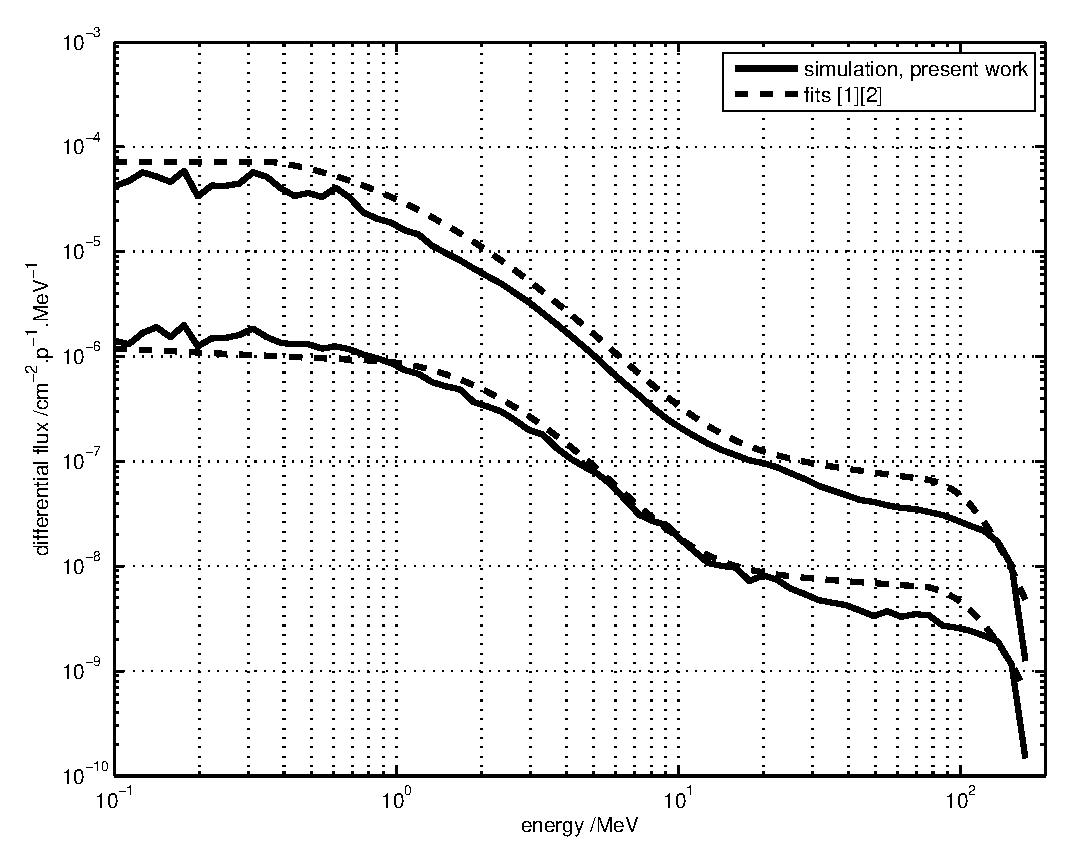
\includegraphics[width=0.9\columnwidth]{DiffYieldComparedSUPCUP10.eps}
    \caption{
        Differential neutron spectra at CUP and SUP (\SI{10.2}{\cm} diameter collimator), comparing results of this work to analytical models~\cite{Prokofiev2009,Prokofiev2014}
    }
    \label{fig:DifferentialSpectra}
\end{figure}

\subsection{Photons}
Fig.~\ref{fig:GammaSpatialDistribution} shows the calculated spatial distribution of gamma photons at SUP and CUP.
Fig.~\ref{fig:DifferentialGammaSpectra} shows the calculated differential gamma spectra within the central region of the spatial distribution.
The results show\ldots
\todo{Describe the gamma results}

\begin{figure}[t]
    \begin{minipage}{\columnwidth}
        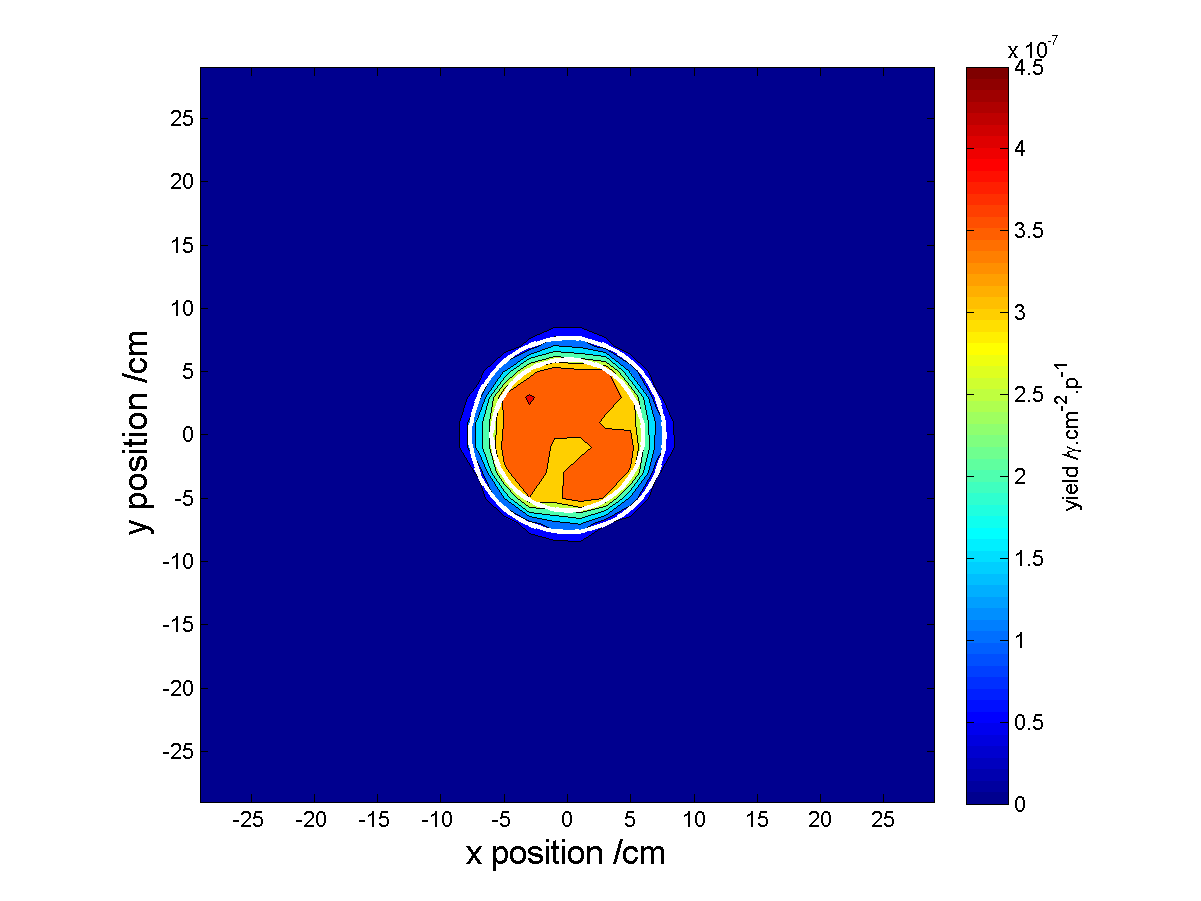
\includegraphics[width=\columnwidth]{SUP10ColSpatialDistributionAllG.png}
        \subcaption{Standard User Position}
        \label{fig:GammaSpatialDistributionSUP}
    \end{minipage}
    \begin{minipage}{\columnwidth}
        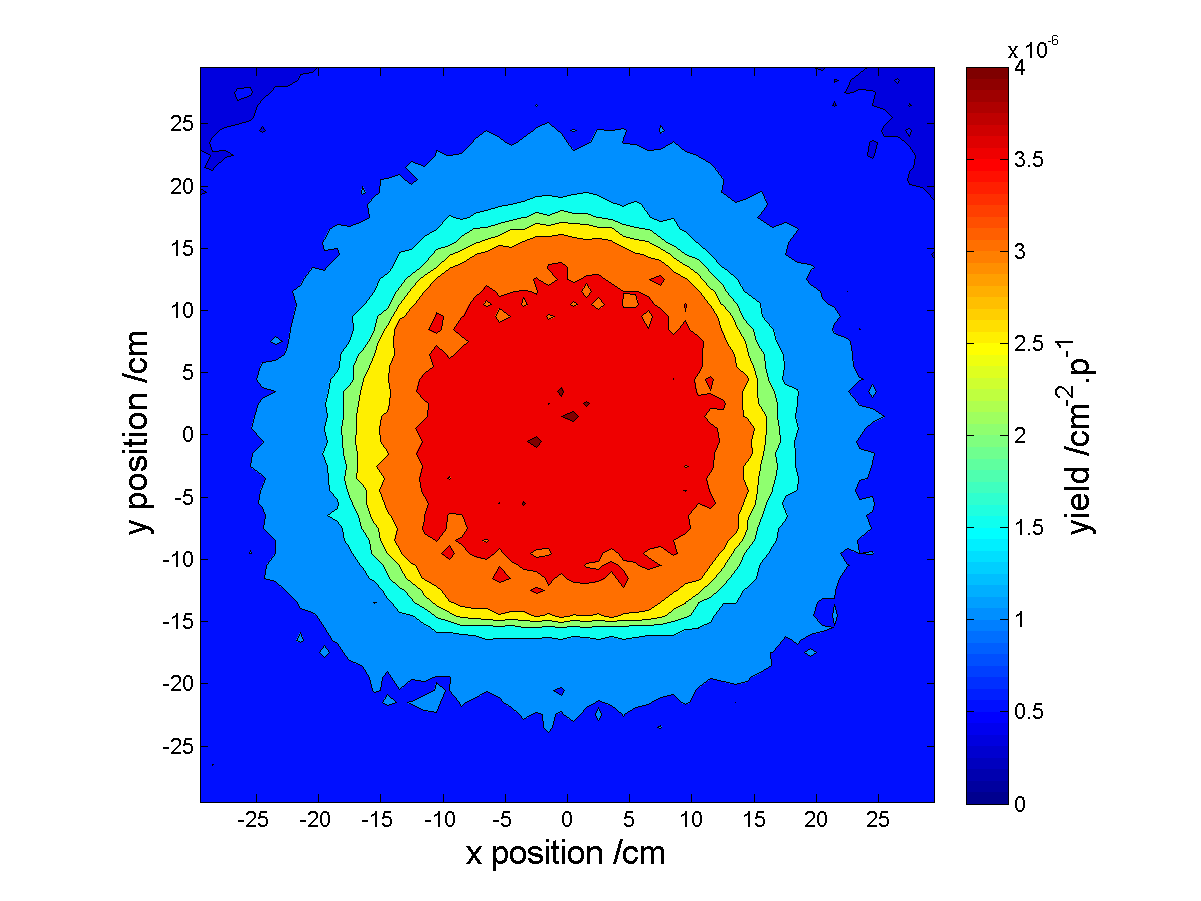
\includegraphics[width=\columnwidth]{CUP10ColSpatialDistributionAllG.png}
        \subcaption{Close User Position}
        \label{fig:GammaSpatialDistributionCUP}
    \end{minipage}
    \caption{
        Calculated gamma spatial distribution, with
        \SI{10.2}{\cm} diameter collimator
    }
    \label{fig:GammaSpatialDistribution}
\end{figure}

\begin{figure}[t]
    \centering
    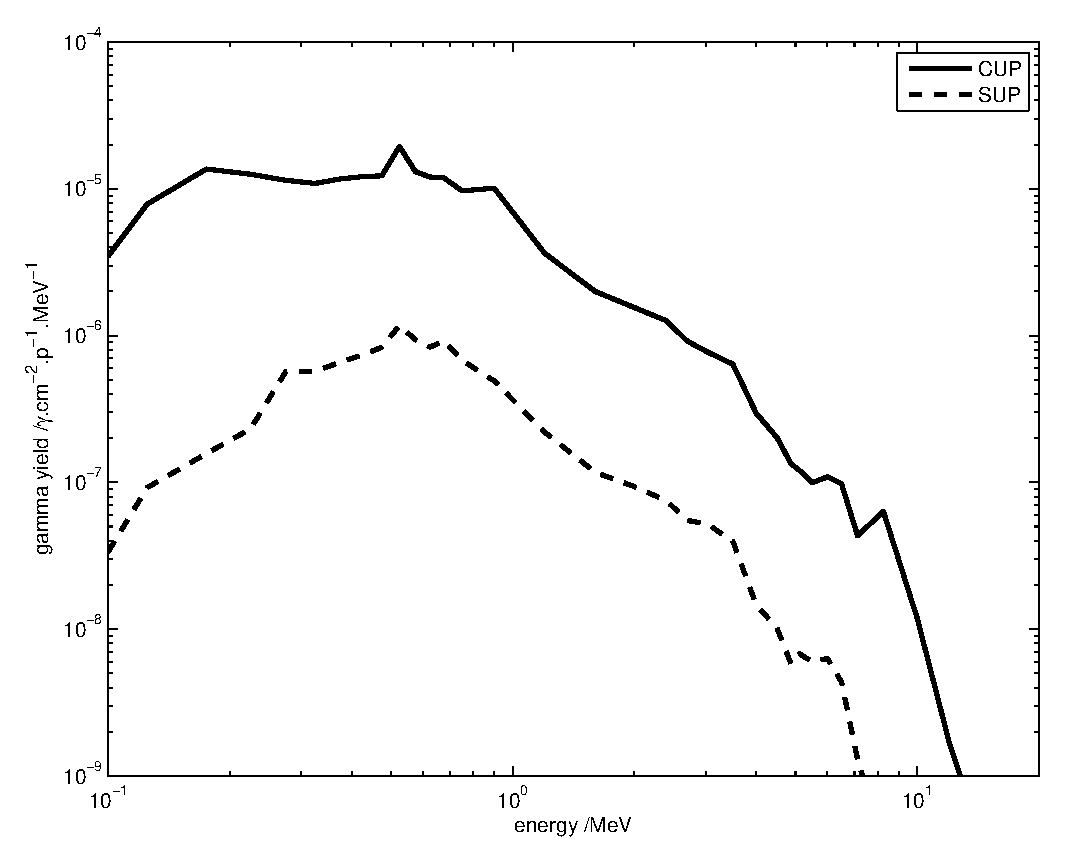
\includegraphics[width=0.9\columnwidth]{gDYieldcomparedRADECS.eps}
    \caption{
        Calculated gamma spectra at CUP and SUP, with
        \SI{10.2}{\cm} diameter collimator
    }
    \label{fig:DifferentialGammaSpectra}
\end{figure}

Fig.~\ref{fig:GammaDoseEnergy} shows the calculated distribution of gamma dose, obtained by folding the gamma spectra (Fig~\ref{fig:GammaDoseEnergy}) with dose conversion data from \cite{Kwon1980}.
The results show\ldots
\todo{Describe the gamma dose versus energy graphs.}
The calculated dose rate at \SI{200}{\nA} primary proton current is \SI{21}{\milli\gray\per\hour} at SUP and \SI{370}{\milli\gray\per\hour} at CUP.
\todo{Discuss calculated dose rates}

\begin{figure}[t]
    \begin{minipage}{\columnwidth}
        \centering
        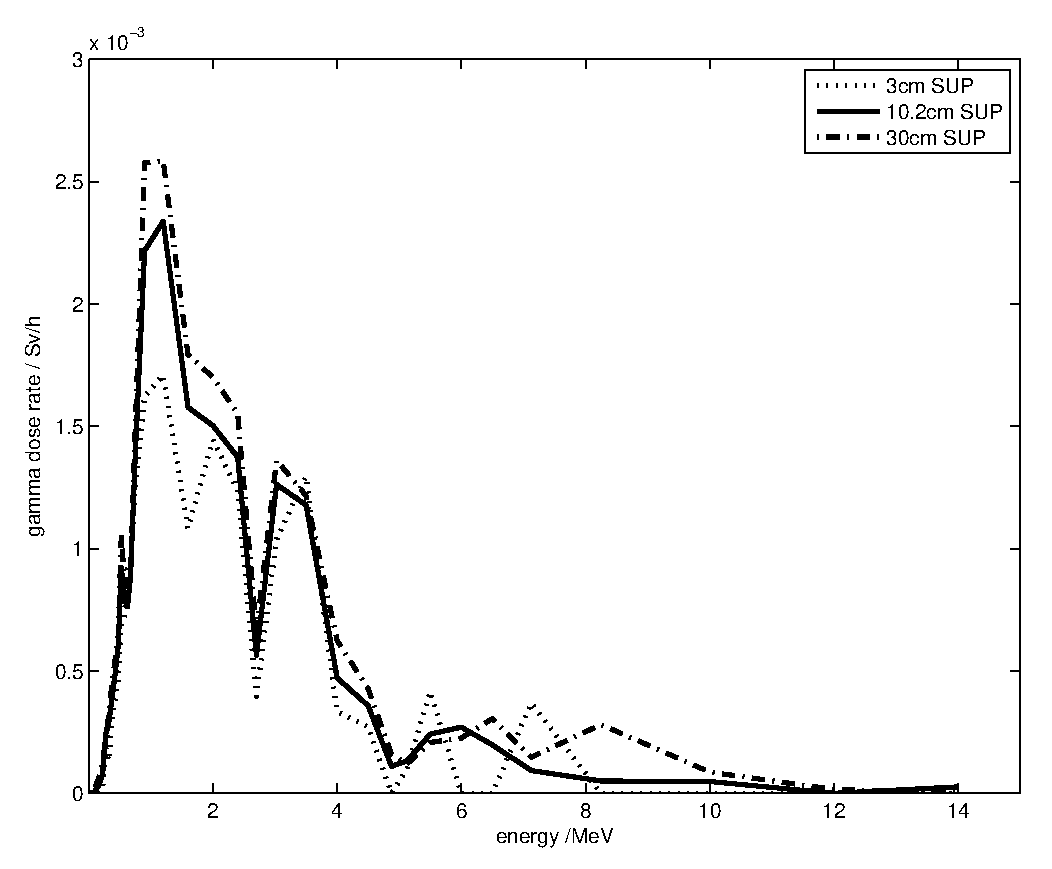
\includegraphics[width=0.9\columnwidth]{DoseVSenergySUP.eps}
        \subcaption{Standard User Position}
        \label{fig:GammaDoseEnergySUP}
    \end{minipage}
    \begin{minipage}{\columnwidth}
        \centering
        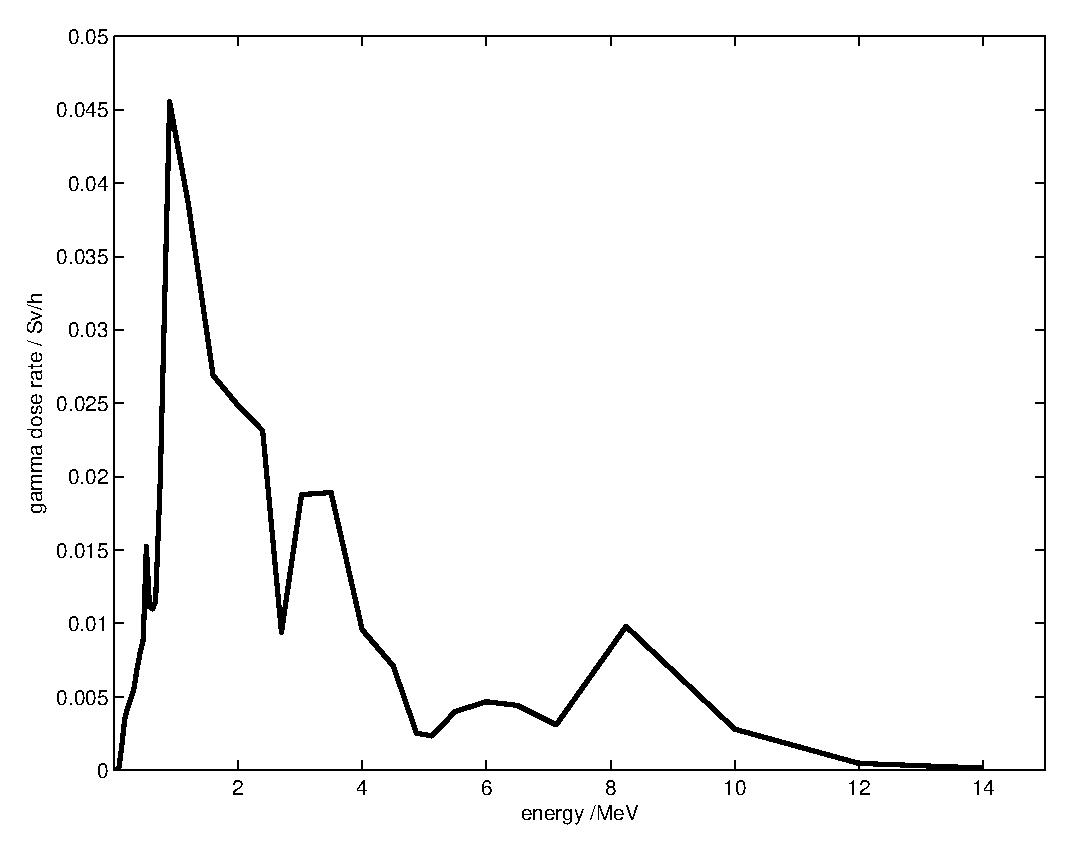
\includegraphics[width=0.9\columnwidth]{DoseVSenergyCUP.eps}
        \subcaption{Close User Position}
        \label{fig:GammaDoseEnergyCUP}
    \end{minipage}
    \caption{
        Calculated gamma dose spectra, with
        \SI{10.2}{\cm} diameter collimator
    }
    \label{fig:GammaDoseEnergy}
\end{figure}

\section{Discussion}
\todo{Discussion}

\begin{thebibliography}{99} % Bibliography - this is intentionally simple in this template

\bibitem{Prokofiev2009}
Prokofiev, A. V. et al.,
\newblock ``Characterization of the ANITA neutron source for accelerated SEE testing at The Svedberg Laboratory'',
\newblock {\em 2009 IEEE Radiat. Effects Data Workshop Record}, pp.~166-173

\bibitem{Prokofiev2014}
Prokofiev, A. V. et al.,
\newblock ``CUP--A new high-flux irradiation position at the ANITA neutron facility at TSL'',		\newblock {\em IEEE Trans. Nucl. Sci.} vol.~61 no.~4, pp.~1929-1936, 2014

\bibitem{Platt2013}
Platt, S. P. et al.,
\newblock ``Neutron and gamma fields at neutron spallation sources for single-event-effects testing'',
\newblock {\em Proc. 14th European Conf. Radiat. Effects Compon. Syst.}, 2013

\bibitem{Agostinelli2003}
Agostinelli, S. et al.,
\newblock``Geant4--a simulation toolkit'',
\newblock {\em Nucl. Inst. Meth. Phys. Res. A} vol.~506, pp.~250--303, 2003

\bibitem{Allison2006}
Allison, J. et al.,
\newblock ``Geant4 developments and applications'',
\newblock {\em IEEE Trans. Nucl. Sci.} vol.~53 no.~1, pp.~270--278, 2006

\bibitem{Carlson2009}
Carlson, A. D. et al.,
\newblock ``International evaluation of neutron cross section standards'',
\newblock{\em Nucl. Data Sheets} vol.~110 no.~12, pp.~3215-3324, 2009

\bibitem{Kwon1980}
Kwon, S.-G. et al.,
\newblock ``Calculation of neutron and gamma-ray flux-to-dose-rate conversion factors'',
\newblock{\em J. Kor. Nucl. Soc.} vol.~12 no.~3, pp.~171-179, 1980

\end{thebibliography}

\cleardoublepage

\todos

\end{document} 